\subsection{Implementation}

The prover is written in Rust~\cite{rust2024} (edition~2024) and consists
of approximately 4{,}500 lines of source code spread over a parser,
abstract-syntax tree, sequent representation, rule applicators, search
engine, and a CLI front-end. The parser is built with
\texttt{pest}~\cite{pest2024}, a parsing-expression-grammar generator,
against a hand-written grammar for the first-order-form (FOF) fragment of
the TPTP language~\cite{Sut17}. The CLI uses
\texttt{clap}~\cite{clap2024} for argument parsing and
\texttt{rusqlite}~\cite{rusqlite2024} for persisting per-problem results
to a SQLite database. Cancellation under \texttt{Ctrl+C} is handled by the
\texttt{ctrlc} crate. The three search engines (\texttt{naive},
\texttt{id}, \texttt{priority-id}) are selected at the command line and
share all code outside the rule scheduler.

Figure~\ref{fig:naive-engine} shows the call structure of the naive
engine.

\begin{figure}
  \centering
  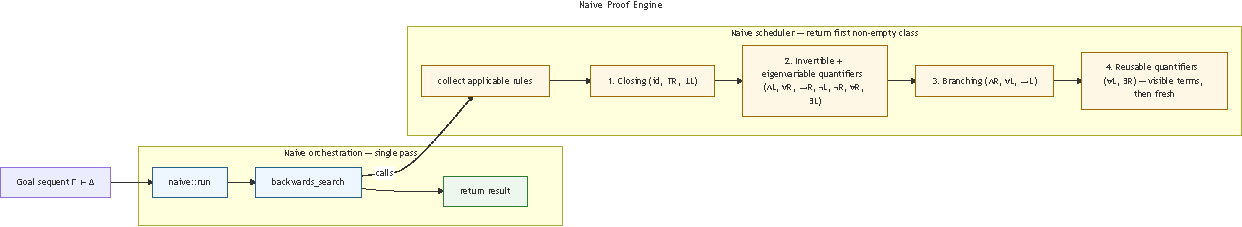
\includegraphics[width=\linewidth]{figures/naive_engine_diagram.pdf}
  \caption{Call structure of the naive proof engine.}
  \label{fig:naive-engine}
\end{figure}

Two design points warrant mention. First, the LK$'$-reusable rules
$\forall L$ and $\exists R$ retain the original quantified formula on its
side of the sequent after instantiation, so the prover tracks per-branch
quantifier-instantiation history (which terms have been used for which
quantified occurrence) to avoid trying the same instantiation twice on the
same branch. Second, fresh-name generation for both eigenconstants
($\forall R$, $\exists L$) and fallback witnesses ($\forall L$, $\exists R$)
inspects every symbol currently visible in the sequent and returns a name
not in that set, guaranteeing eigenvariable freshness without further
$\alpha$-renaming machinery. Substitution is capture-avoiding by
construction because only ground terms are ever instantiated for bound
variables.
